\documentclass[12pt,a4paper]{report}

\usepackage[utf8]{inputenc}
\usepackage[T1]{fontenc}
\usepackage[english]{babel}
\usepackage{geometry}
\geometry{margin=2.5cm}

\usepackage{listings}
\usepackage{xcolor}
\usepackage{graphicx}
\usepackage{booktabs}
\usepackage{hyperref}
\usepackage{todonotes}
\usepackage{caption}
\usepackage{subcaption}
\usepackage{float}
\usepackage{amsmath}
\usepackage{multirow}

% ------------------------------------------------------------------
% C listing style with OpenMP keywords highlighted
% ------------------------------------------------------------------
\definecolor{codegreen}{rgb}{0,0.5,0}
\definecolor{codegray}{rgb}{0.5,0.5,0.5}
\definecolor{codeblue}{rgb}{0,0,0.8}
\definecolor{codepurple}{rgb}{0.5,0,0.5}
\definecolor{backcolour}{rgb}{0.97,0.97,0.97}

\lstdefinestyle{cstyle}{
    language=C,
    backgroundcolor=\color{backcolour},
    basicstyle=\ttfamily\footnotesize,
    keywordstyle=\color{codeblue}\bfseries,
    commentstyle=\color{codegreen}\itshape,
    stringstyle=\color{codepurple},
    numberstyle=\tiny\color{codegray},
    numbers=left,
    stepnumber=1,
    numbersep=6pt,
    showspaces=false,
    showstringspaces=false,
    tabsize=4,
    frame=single,
    breaklines=true,
    breakatwhitespace=true,
    captionpos=b,
    morekeywords={pragma,omp,parallel,single,task,taskgroup,taskwait,
                  firstprivate,shared,private,reduction,atomic,critical,
                  if,final,depend,untied,mergeable,priority},
}
\lstset{style=cstyle}

% ------------------------------------------------------------------
% Metadata
% ------------------------------------------------------------------
\title{%
    \textbf{PAR Laboratory Assignment}\\[0.4em]
    \large Lab 4: Parallel Task Decomposition\\
    Implementation and Analysis%
}
\author{%
    Oriol Valencia\\[0.4em]
    \small Universitat Polit\`{e}cnica de Catalunya\\
    \small Departament d'Arquitectura de Computadors%
}
\date{Spring 2025--2026}

% ------------------------------------------------------------------
\begin{document}

\maketitle
\tableofcontents
\newpage

% ==================================================================
\chapter{Iterative Task Decomposition}
% ==================================================================

% ==================================================================
\section{Iterative: Tile Task Decomposition}
\label{sec:iter-tile}
% ==================================================================

\subsection{Implementation}
\label{sec:iter-tile-impl}

The \textbf{original tile iterative} strategy maps the $\mathit{ROWS}\times\mathit{COLS}$ image
onto a grid of square tiles of size $\mathit{TILE}\times\mathit{TILE}$ pixels.
The outer double loop iterates over tile origins with stride \texttt{TILE}; each iteration
body is wrapped in a single \texttt{\#pragma~omp~task}, so all tiles are eligible for
parallel execution.
The task takes \texttt{x} and \texttt{y} as \texttt{firstprivate} to avoid the data-race
that would arise if the loop variables were shared across concurrently executing tasks.

The parallel region is opened with \texttt{\#pragma~omp~parallel} followed immediately by
\texttt{\#pragma~omp~single}, so only one thread generates the tasks while all others
are available to execute them.

\begin{lstlisting}[caption={Key parallel section of \texttt{mandel-omp-iter.c} (Tile strategy).},
                   label={lst:iter-tile}]
#pragma omp parallel
#pragma omp single
for (int y = 0; y < ROWS; y += TILE)
    for (int x = 0; x < COLS; x += TILE) {
        #pragma omp task firstprivate(x, y)
        {
            int equal = 1;
            // --- Check vertical TILE borders ---
            int ref = pixel_dwell(..., x, y, ...);
            for (int py = y; py < y + TILE; py++) {
                M[py][x]          = pixel_dwell(..., x,          py, ...);
                M[py][x+TILE-1]   = pixel_dwell(..., x+TILE-1,  py, ...);
                equal &= (ref == M[py][x]);
                equal &= (ref == M[py][x+TILE-1]);
            }
            // --- Check horizontal TILE borders ---
            for (int px = x; px < x + TILE; px++) {
                M[y][px]          = pixel_dwell(..., px, y,         ...);
                M[y+TILE-1][px]   = pixel_dwell(..., px, y+TILE-1, ...);
                equal &= (ref == M[y][px]);
                equal &= (ref == M[y+TILE-1][px]);
            }
            if (equal) {
                fill_tile(M, y, x, TILE, M[y][x]);   // uniform colour
            } else {
                compute_tile(M, y, x, TILE, ...);     // full computation
            }
        }
    }
\end{lstlisting}

Dependencies and data-sharing between tasks are avoided by construction: each task writes
only to the memory region $[y,\,y+\mathit{TILE})\times[x,\,x+\mathit{TILE})$, which is
disjoint from every other task's region.
Histogram updates use \texttt{\#pragma~omp~atomic} to protect the shared counter array.

\subsection{Modelfactor Analysis}
\label{sec:iter-tile-mf}

% TODO: Run  sbatch submit-strong-extrae.sh mandel-omp-iter
%       and paste the Modelfactors tables here.

\todo[inline]{Insert Modelfactors table for \texttt{mandel-omp-iter} (16 threads) and
identify the main bottlenecks (e.g.\ scheduling overhead, load imbalance, synchronisation).}

% Example skeleton (replace values with real data):
% \begin{table}[H]
% \centering
% \caption{Modelfactors for Iterative Tile with 16 threads.}
% \begin{tabular}{lr}
% \toprule
% Factor & Value \\
% \midrule
% Useful computation & \% \\
% Task scheduling overhead & \% \\
% Synchronisation & \% \\
% \bottomrule
% \end{tabular}
% \end{table}
%
% Main issues observed:
% - ...

\subsection{Paraver Analysis}
\label{sec:iter-tile-paraver}

% TODO: Open the Paraver trace generated for 16 threads and include:
%   1. The "Useful/Instantaneous parallelism" view.
%   2. The "OpenMP tasking / explicit tasks function created and executed" view.

\todo[inline]{Insert Paraver screenshots (16 threads) and comment on the task creation
pattern, load distribution, and any visible idle periods.}

% \begin{figure}[H]
%   \centering
%   \includegraphics[width=\linewidth]{fotos/iter-tile-paraver-parallelism.png}
%   \caption{Useful/Instantaneous parallelism -- Iterative Tile, 16 threads.}
%   \label{fig:iter-tile-paraver}
% \end{figure}

\subsection{Strong Scalability}
\label{sec:iter-tile-scalability}

% TODO: Run  sbatch submit-strong-omp.sh  and include the speedup plot.

\todo[inline]{Insert the strong scalability (speedup vs.\ number of threads) plot for
\texttt{mandel-omp-iter} and explain the observed trend.}

% \begin{figure}[H]
%   \centering
%   \includegraphics[width=0.75\linewidth]{fotos/iter-tile-speedup.png}
%   \caption{Strong scalability of Iterative Tile.}
%   \label{fig:iter-tile-speedup}
% \end{figure}

\clearpage
% ==================================================================
\section{Iterative: Fine Grain Task Decomposition}
\label{sec:iter-fine}
% ==================================================================

\subsection{Implementation}
\label{sec:iter-fine-impl}

The \textbf{fine grain iterative} strategy extends the Tile version by exploiting the
additional parallelism that exists \emph{inside} each tile.
Rather than completing the border check and fill/compute sequentially within each tile
task, the fine grain version exposes three independent sub-tasks per tile:

\begin{enumerate}
    \item A task that computes the \emph{vertical} borders of the tile (left and right
          columns), setting \texttt{eV}.
    \item A task that computes the \emph{horizontal} borders (top and bottom rows,
          including all four corners), setting \texttt{eH}.
    \item A task (spawned after \texttt{\#pragma~omp~taskgroup} ensures both border tasks
          have finished) that either fills the tile uniformly or, in the non-uniform case,
          spawns one child task per row to compute all interior pixels.
\end{enumerate}

The outer tile task from the Tile version is \textbf{kept} as a wrapper; the three inner
tasks are created inside it.

\begin{lstlisting}[caption={Key parallel section of \texttt{fine-grain.c} -- inner tasks
                   for each tile.}, label={lst:fine-grain}]
#pragma omp parallel
#pragma omp single
for (int y = 0; y < ROWS; y += TILE)
    for (int x = 0; x < COLS; x += TILE) {
        #pragma omp task firstprivate(x, y)
        {
            int eV, eH;

            #pragma omp taskgroup
            {
                // Task 1: vertical borders (left & right columns)
                #pragma omp task shared(eV)
                {
                    eV = 1;
                    int ref = pixel_dwell(..., x, y, ...);
                    for (int py = y; py < y + TILE; py++) {
                        M[py][x]        = pixel_dwell(..., x,        py, ...);
                        M[py][x+TILE-1] = pixel_dwell(..., x+TILE-1, py, ...);
                        eV &= (ref == M[py][x]);
                        eV &= (ref == M[py][x+TILE-1]);
                    }
                }
                // Task 2: horizontal borders (top & bottom rows)
                #pragma omp task shared(eH)
                {
                    eH = 1;
                    for (int px = x; px < x + TILE; px++) {
                        M[y][px]        = pixel_dwell(..., px, y,        ...);
                        M[y+TILE-1][px] = pixel_dwell(..., px, y+TILE-1, ...);
                        eH &= (M[y][x] == M[y][px]);
                        eH &= (M[y][x] == M[y+TILE-1][px]);
                    }
                }
            } // implicit taskwait -- eH and eV are ready here

            // Task 3: fill or compute (spawns per-row child tasks)
            #pragma omp task
            {
                if (eH & eV) {                       // uniform tile
                    for (int py = y; py < y + TILE; py++)
                        #pragma omp task
                        fill_row(M, py, x, TILE, M[y][x], ...);
                } else {                             // non-uniform tile
                    for (int py = y; py < y + TILE; py++)
                        #pragma omp task
                        compute_row(M, py, x, TILE, ...);
                }
            }
        }
    }
\end{lstlisting}

The \texttt{\#pragma~omp~taskgroup} enforces that the result tasks begin only after
\emph{both} border tasks complete, because the fill/compute decision depends on
\texttt{eV} and \texttt{eH}.
Histogram increments remain protected by \texttt{\#pragma~omp~atomic}.
Display updates use \texttt{\#pragma~omp~critical} to serialize X11 calls.

\paragraph{Comparison with Iterative Tile.}
The Tile version creates $\bigl(\mathit{ROWS}/\mathit{TILE}\bigr)^{2}$ tasks in total.
The Fine Grain version creates up to $3 + 2\cdot\mathit{TILE}$ tasks \emph{per tile},
increasing the task count by roughly $2\cdot\mathit{TILE}$ fold.
This exposes more parallelism at the cost of higher task-creation and synchronisation
overhead; whether the trade-off is beneficial depends on tile size and thread count.

\subsection{Modelfactor Analysis}
\label{sec:iter-fine-mf}

% TODO: Run  sbatch submit-strong-extrae.sh mandel-omp-fine-grain
%       Paste Modelfactors tables and compare with the Tile version.

\todo[inline]{Insert Modelfactors table for \texttt{fine-grain} (16 threads).
Compare with Iterative Tile: does finer granularity improve useful parallelism or does
scheduling overhead dominate?}

\subsection{Paraver Analysis}
\label{sec:iter-fine-paraver}

% TODO: Include Paraver views for 16 threads and compare with Iterative Tile.
%   - "Useful/Instantaneous parallelism"
%   - "OpenMP tasking / explicit tasks function created and executed"
%   Compare task density, idle gaps, and load balance with the Tile trace.

\todo[inline]{Insert Paraver screenshots (16 threads) for Fine Grain and compare with
the Tile trace. Comment on whether the extra tasks reduce idle time or introduce
additional overhead.}

% \begin{figure}[H]
%   \centering
%   \begin{subfigure}[b]{0.48\linewidth}
%     \includegraphics[width=\linewidth]{fotos/iter-tile-paraver-tasks.png}
%     \caption{Iterative Tile.}
%   \end{subfigure}
%   \hfill
%   \begin{subfigure}[b]{0.48\linewidth}
%     \includegraphics[width=\linewidth]{fotos/iter-fine-paraver-tasks.png}
%     \caption{Iterative Fine Grain.}
%   \end{subfigure}
%   \caption{Task creation view -- 16 threads.}
%   \label{fig:fine-paraver-compare}
% \end{figure}

\subsection{Strong Scalability}
\label{sec:iter-fine-scalability}

% TODO: Include speedup plot and compare with Iterative Tile.

\todo[inline]{Insert the strong scalability plot for Fine Grain and compare with
the Tile speedup curve. Discuss whether additional task granularity improves
or hurts scalability at high thread counts.}

% \begin{figure}[H]
%   \centering
%   \includegraphics[width=0.75\linewidth]{fotos/iter-fine-speedup.png}
%   \caption{Strong scalability comparison: Iterative Tile vs.\ Fine Grain.}
%   \label{fig:fine-speedup}
% \end{figure}

\clearpage

% ==================================================================
\chapter{Recursive Task Decomposition}
% ==================================================================

% ==================================================================
\section{Recursive: Leaf Task Decomposition}
\label{sec:rec-leaf}
% ==================================================================

\subsection{Implementation}
\label{sec:rec-leaf-impl}
El codi de la versió \textbf{leaf recursive} es troba a \texttt{mandel-omp-leaf.c}.\\
El primer que analitzarem és que la regió paral·lela es crea al main, abans de la crida a \texttt{mandel\_tiled\_rec}, declarant la regió com a \texttt{single}. Això provocarà que un únic thread crei les tasques i faci el recorregut recursiu (és com funciona l'estratègia \textbf{leaf}).

\begin{lstlisting}[caption={Regió paral·lela i crida inicial al \texttt{main}.},label={lst:rec-leaf-main}]
#pragma omp parallel
#pragma omp single
mandel_tiled_rec((int (*)[width])Hmatrix, height, width, 0, 0,
             real_min, imag_min, real_max, imag_max,
             scale_real, scale_imag, maxiter);
\end{lstlisting}

Posteriorment, veiem que només es creen tasques a les fulles de l'arbre de recursió, en dos casos. O bé quan \texttt{equal} és cert, és a dir, les boreres del tile són iguals i es pot omplir el tile amb un valor uniforme, o bé quan el nombre de columnes és menor o igual que la mida del tile, cosa que indica que s'ha arribat a un tile prou petit perquè es calculi directament. En ambdós casos es crea una tasca per dur a terme l'operació corresponent. Vegeu-ho al propi codi, no s'adjunta perquè cada cas base ocupa moltes línies.\\
Si no es compleix cap de les condicions anteriors, la recursió es fa als quatre quadrants del tile (o a les dues meitats de columnes), però sense crear tasques per a aquestes crides recursives, cosa característica de l'estratègia \textbf{leaf}.\\
Cal destacar també que s'han evitat els problemes de compartició de dades en els accessos a l'histograma i a la biblioteca X detectats a la pràctica 3, de la manera següent:
\begin{itemize}
    \item Per l'accès a histograma, s'ha utilitzat \texttt{\#pragma omp atomic}:
    \begin{lstlisting}[language=C]
#pragma omp atomic
histogram[M[y][x] - 1] += (NRows * NCols);
    \end{lstlisting}

    \item Per l'accès a la librería X, las instruccions s'han protegit amb \texttt{\#pragma omp critical}:
    \begin{lstlisting}[language=C]
#pragma omp critical
{
    XSetForeground(display, gc, color);
    XDrawPoint(display, win, gc, px, py);
}
    \end{lstlisting}
\end{itemize}

\subsection{Modelfactor Analysis}
\label{sec:rec-leaf-mf}

% Modelfactors tables (three model factors)
% Mostrar las tres tablas de modelfactor verticalmente, cada una más grande
\begin{figure}[H]
    \centering
    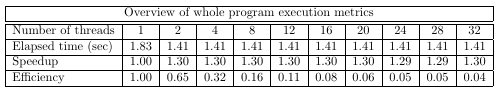
\includegraphics[width=0.9\linewidth]{fotosL4/primera_tabla_leaf.png}
    \caption{Model factor 1 (Leaf).}
    \label{fig:rec-leaf-mf1}
\end{figure}

\begin{figure}[H]
    \centering
    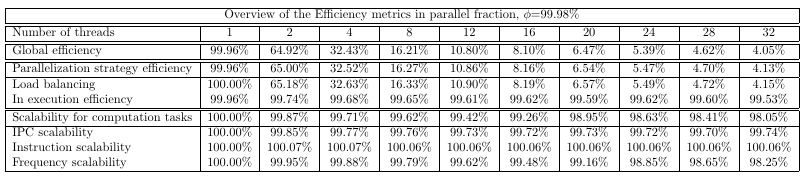
\includegraphics[width=0.9\linewidth]{fotosL4/segunda_tabla_leaf.png}
    \caption{Model factor 2 (Leaf).}
    \label{fig:rec-leaf-mf2}
\end{figure}

\begin{figure}[H]
    \centering
    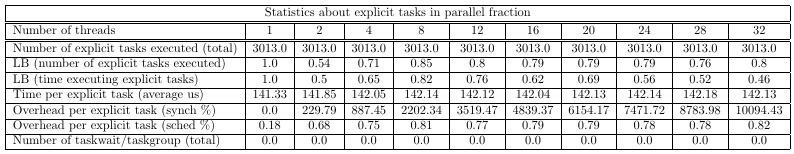
\includegraphics[width=0.9\linewidth]{fotosL4/tercera_tabla_leaf.png}
    \caption{Model factor 3 (Leaf).}
    \label{fig:rec-leaf-mf3}
\end{figure}
A la primera de les taules podem veure diversos aspectes que ens reflecteixen que no serà una implementació "molt bona". Veiem que l'Elapsed time, no baixa a partir de l'execució amb 2 threads amb un valor de 1.41 s, i que el Speedup no millora a partir de 2 threads, mantenint-se al voltant de 1.3. Això es veu reflectit en una eficiència molt baixa.\\
Això es deu a què el coll d'ampolla en aquest cas és la creació de tasques, que es fa de manera serial, i això provoca que la resta de threads estiguin inactius durant aquest procés. Per tant una execució amb 2 threads ja és suficient per mantenir ocupat el thread que crea les tasques i un altre que les executa, i afegir més threads no aporta cap millora.
Veiem a la taula 2 que el load balancing no es bo. Amb 2 threads és de 65\% i cau fins al 4.15\%, reduint-se a la meitar al duplicar el nombre de threads. Això es deu a la desigualtat en la creació de tasques, i a què hi ha tasques que tenen més cost que d'altres, els tiles de l'interior, i això provoca desequilibris.\\
De la tercera taula es destaca el nombre de tasques executades, que és 3013. Es compararà amb el nombre de tasques creat en altres apartats.

\subsection{Paraver Analysis}
\label{sec:rec-leaf-paraver}

% Paraver trace (useful/instantaneous parallelism and task creation view)
\begin{figure}[H]
    \centering
    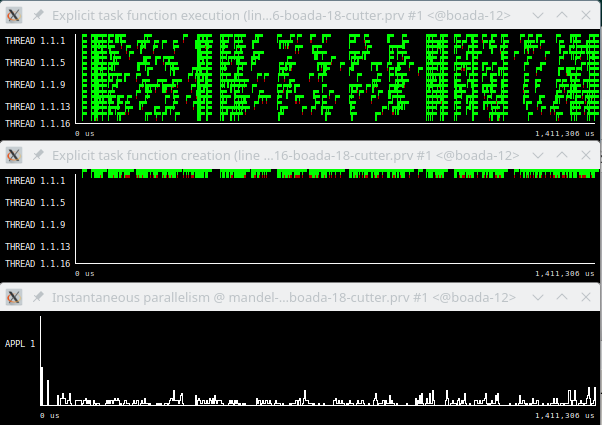
\includegraphics[width=0.9\linewidth]{fotosL4/paraver_leaf.png}
    \caption{Paraver trace for Recursive Leaf (16 threads): task creation and useful parallelism.}
    \label{fig:rec-leaf-paraver}
\end{figure}

A les traces obtingudes de Paraver, es pot observar, d'una banda, que la creació de tasques es fa únicament en un fil, i que la resta de fils es mantenen inactius fins que aquestes tasques es creen i s'assignen. Això es concorde amb l'anàlisi fet a la pràctica 3, on es va observar un desequilibri de càrrega entre la creació de tasques i la seva execució.
Podem veure però, que a l'hora de l'execució de les tasques, els 16 threads es mantenen actius, el que indica que la paralelització a nivell de tasques és efectiva un cop les tasques han estat creades.
A la tercera traça, es reflexa que el pararelisme és molt irregular, amb períodes de paralelisme útils seguits de períodes d'inactivitat. Això es deu a què, d'una banda a l'estratègia leaf no es creen totes les tasques a l'hora, i hi ha moments on no hi ha tasques disponibles per executar. D'altra banda, hi ha tasques que tenen més cost que d'altres, els tiles de l'interior, i això també provoca desequilibris.
Tot això reflexa la baixa eficiència del model de tasques en aquesta implementació, ja que 15 dels 16 threads estan inactius durant la creació de tasques i només es mantenen ocupats una vegada que les tasques han estat creades, i ho fan de manera irregular.

\subsection{Strong Scalability}
\label{sec:rec-leaf-scalability}

% Strong scalability plot
\begin{figure}[H]
    \centering
    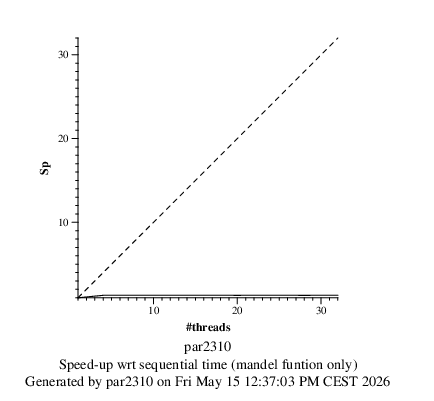
\includegraphics[width=0.75\linewidth]{fotosL4/grafico_leaf.png}
    \caption{Strong scalability (elapsed time vs. threads) for the Recursive Leaf implementation.}
    \label{fig:rec-leaf-speedup}
\end{figure}

De la figura prèvia en podem analitzar que l'increment de l'SpeedUp en relació al nombre de threads és nul, com ja haviem vist amb les taules modelfactor. Si que hi ha un increment de l'SpeedUp quan es passa de 1 a 2 threads, però a partir d'aquí no hi ha cap millora, mantenint-se al voltant de 1.3.\\

\clearpage
% ==================================================================
\section{Recursive: Improved Leaf Task Decomposition}
\label{sec:rec-improved}
% ==================================================================

\subsection{Implementation}
\label{sec:rec-improved-impl}

The \textbf{improved leaf} version addresses the main bottleneck of the plain leaf
strategy: serial task generation.
In the leaf version, the entire recursion is driven by a single thread, so threads
sit idle until enough leaf tasks have accumulated.
The improvement introduces a \emph{depth cutoff} parameter \texttt{d} (initialised to
\texttt{0} at the top-level call) and a compile-time constant \texttt{CUTOFF}.

\begin{itemize}
    \item When the current recursion depth satisfies $\mathtt{d} < \mathtt{CUTOFF}$,
          each recursive quadrant call is wrapped in a \texttt{\#pragma~omp~task},
          allowing multiple threads to explore different branches of the recursion tree
          \emph{concurrently}.
    \item When $\mathtt{d} \ge \mathtt{CUTOFF}$, the recursive calls are sequential
          again, cutting off task proliferation at deep levels where the overhead would
          dominate.
    \item Leaf tasks (fill or compute) are only spawned when $\mathtt{d} \le
          \mathtt{CUTOFF}$; beyond the cutoff they run inline to avoid the overhead of
          tiny tasks.
\end{itemize}

The value \texttt{CUTOFF = 16} was chosen empirically so that the number of tasks at
the cutoff level matches or exceeds the number of available threads.

\begin{sloppypar}
The complete implementation (depth-cutoff mechanism with \texttt{CUTOFF = 16}) is in \path{codis/leaf-improved.c}.
\end{sloppypar}

The \texttt{\#pragma~omp~taskgroup} ensures that all four quadrant tasks (and their
descendants) finish before control returns to the caller, preserving the border-read
correctness that the leaf version relies on.

\paragraph{Improvements over plain Leaf.}
\begin{itemize}
    \item Multiple threads now explore the recursion tree in parallel down to depth
          \texttt{CUTOFF}, eliminating the serial task-generation bottleneck.
    \item Tasks beyond \texttt{CUTOFF} run sequentially, avoiding excessive fine-grained
          task overhead at the bottom of the tree.
    \item The result is speedups larger than $2\times$ for more than 2 threads.
\end{itemize}

\subsection{Modelfactor Analysis}
\label{sec:rec-improved-mf}

Tables~\ref{tab:li-exec}--\ref{tab:li-tasks} summarise the Modelfactors output for
\texttt{mandel-omp-rec-improved-leaf} obtained on \texttt{par2317}.

\begin{table}[h]
\resizebox{\textwidth}{!}{%
\begin{tabular}{|l|c|c|c|c|c|c|c|c|c|c|}
\hline
\multicolumn{11}{|c|}{Overview of whole program execution metrics} \\
\hline
\hline
Number of threads & 1 & 2 & 4 & 8 & 12 & 16 & 20 & 24 & 28 & 32 \\
\hline
Elapsed time (sec)      &       1.82 &       0.99 &       0.58 &       0.38 &       0.38 &       0.38 &       0.38 &       0.38 &       0.38 &       0.38 \\
\hline
Speedup                 &       1.00 &       1.84 &       3.12 &       4.76 &       4.76 &       4.74 &       4.74 &       4.74 &       4.73 &       4.74 \\
\hline
Efficiency              &       1.00 &       0.92 &       0.78 &       0.60 &       0.40 &       0.30 &       0.24 &       0.20 &       0.17 &       0.15 \\
\hline
\end{tabular}
}
\caption{Improved Leaf -- whole program execution metrics. Analysis: par2317, 2026-05-15.}
\label{tab:li-exec}
\end{table}


\begin{table}[h]
\resizebox{\textwidth}{!}{%
\begin{tabular}{|l|c|c|c|c|c|c|c|c|c|c|}
\hline
\multicolumn{11}{|c|}{Overview of the Efficiency metrics in parallel fraction, $\phi$=99.98\%} \\
\hline
\hline
Number of threads & 1 & 2 & 4 & 8 & 12 & 16 & 20 & 24 & 28 & 32 \\
\hline
\hline
Global efficiency                      &     99.96\% &     91.86\% &     77.89\% &     59.57\% &     39.63\% &     29.65\% &     23.69\% &     19.77\% &     16.91\% &     14.81\% \\
\hline
\hline
Parallelization strategy efficiency &     99.96\% &     92.02\% &     78.01\% &     59.70\% &     39.78\% &     29.83\% &     23.91\% &     20.00\% &     17.18\% &     15.11\% \\
\hline
Load balancing                   &    100.00\% &     92.07\% &     80.14\% &     66.58\% &     45.42\% &     31.87\% &     27.40\% &     22.91\% &     18.37\% &     17.31\% \\
In execution efficiency          &     99.96\% &     99.94\% &     97.34\% &     89.66\% &     87.57\% &     93.59\% &     87.25\% &     87.31\% &     93.54\% &     87.31\% \\
\hline
\hline
Scalability for computation tasks   &    100.00\% &     99.83\% &     99.85\% &     99.78\% &     99.63\% &     99.40\% &     99.10\% &     98.82\% &     98.42\% &     98.04\% \\
\hline
IPC scalability                  &    100.00\% &     99.94\% &     99.95\% &     99.97\% &     99.94\% &     99.92\% &     99.90\% &     99.93\% &     99.93\% &     99.91\% \\
Instruction scalability          &    100.00\% &    100.00\% &    100.00\% &    100.00\% &    100.00\% &    100.00\% &    100.00\% &    100.00\% &    100.00\% &    100.00\% \\
Frequency scalability            &    100.00\% &     99.89\% &     99.89\% &     99.82\% &     99.68\% &     99.48\% &     99.19\% &     98.89\% &     98.49\% &     98.12\% \\
\hline
\end{tabular}
}
\caption{Improved Leaf -- efficiency breakdown ($\phi$=99.98\%). Analysis: par2317, 2026-05-15.}
\label{tab:li-efficiency}
\end{table}


\begin{table}[h]
\resizebox{\textwidth}{!}{%
\begin{tabular}{|l|c|c|c|c|c|c|c|c|c|c|}
\hline
\multicolumn{11}{|c|}{Statistics about explicit tasks in parallel fraction} \\
\hline
\hline
Number of threads & 1 & 2 & 4 & 8 & 12 & 16 & 20 & 24 & 28 & 32 \\
\hline
\hline
Number of explicit tasks executed (total)        &            66.0 &            66.0 &            66.0 &            66.0 &            66.0 &            66.0 &            66.0 &            66.0 &            66.0 &            66.0 \\
\hline
LB (number of explicit tasks executed)           &             1.0 &            0.87 &            0.69 &            0.49 &            0.55 &            0.59 &            0.55 &            0.55 &            0.47 &            0.55 \\
\hline
LB (time executing explicit tasks)               &             1.0 &            0.93 &            0.79 &            0.69 &            0.55 &            0.47 &             0.4 &             0.3 &            0.24 &            0.27 \\
\hline
Time per explicit task (average us)                 &        27349.36 &        27384.63 &        27386.04 &        28433.09 &        34192.49 &        40782.88 &        41755.11 &        37641.56 &        37773.34 &        41457.39 \\
\hline
Overhead per explicit task (synch \%)             &            0.04 &            8.71 &           28.37 &           65.43 &          122.21 &          159.14 &          210.86 &          295.23 &          355.38 &          379.16 \\
\hline
Overhead per explicit task (sched \%)             &             0.0 &             0.0 &            0.01 &            0.01 &            0.02 &            0.01 &            0.02 &            0.01 &            0.02 &            0.02 \\
\hline
Number of taskwait/taskgroup (total)             &          1004.0 &          1004.0 &          1004.0 &          1004.0 &          1004.0 &          1004.0 &          1004.0 &          1004.0 &          1004.0 &          1004.0 \\
\hline
\end{tabular}
}
\caption{Improved Leaf -- explicit task statistics. Analysis: par2317, 2026-05-15.}
\label{tab:li-tasks}
\end{table}


\paragraph{Observations.}
The improved leaf version exposes a clear performance ceiling.
Elapsed time decreases from 1.82\,s (1 thread) to 0.38\,s at 8 threads
(speedup $4.76\times$) and then remains \emph{flat} all the way to 32 threads
(Table~\ref{tab:li-exec}).
Efficiency collapses to 15\,\% at 32 threads.

The efficiency breakdown (Table~\ref{tab:li-efficiency}) identifies \emph{load
imbalance} as the dominant bottleneck: the load-balancing factor falls from 100\,\% at
1 thread to only 17.31\,\% at 32 threads.
This is a direct consequence of the small total task count: only \textbf{66 explicit
tasks} are generated (Table~\ref{tab:li-tasks}), making it impossible to distribute
work evenly across more than a handful of threads.

The synchronisation overhead per task tells the same story:
it grows from 0.04\,\% at 1 thread to \textbf{379\,\%} at 32 threads, meaning threads
spend nearly four times as long waiting at synchronisation points (\texttt{taskwait}/
\texttt{taskgroup}) as they do executing useful computation.
This is caused by the 1\,004 \texttt{taskwait}/\texttt{taskgroup} operations that must
serialise access between recursion levels, each becoming a bottleneck when more threads
contend for a small pool of tasks.
Scheduling overhead, by contrast, is negligible ($\leq$0.02\,\%), confirming that the
overhead is synchronisation-bound, not dispatch-bound.

\begin{sloppypar}
The saturation at 8 threads matches the CUTOFF-induced task count: with \texttt{CUTOFF=16},
the recursion tree generates at most $4^{\lceil\log_4 66\rceil}$ leaf tasks, and at 8
threads the work is fully distributed; additional threads find no tasks and remain idle.
\end{sloppypar}

Compared with the plain Leaf version, the improved leaf eliminates the serial
task-generation phase (multiple threads now traverse the recursion tree in parallel up
to the cutoff), but the fundamental limit of 66 tasks prevents further scaling beyond
8 threads.
Increasing \texttt{CUTOFF} would generate more tasks and potentially improve scalability
at the cost of higher synchronisation overhead per task.

\subsection{Paraver Analysis}
\label{sec:rec-improved-paraver}

% TODO: Include Paraver views for 16 threads.
%   Compare with the plain Leaf trace:
%   - Is the initial serial phase shorter or eliminated?
%   - Is load balance better?

\todo[inline]{Insert Paraver screenshots (16 threads) for Improved Leaf.
Include both the non-improved and the improved traces for direct comparison.}

% \begin{figure}[H]
%   \centering
%   \begin{subfigure}[b]{0.48\linewidth}
%     \includegraphics[width=\linewidth]{fotos/rec-leaf-paraver-parallelism.png}
%     \caption{Plain Leaf -- parallelism view.}
%   \end{subfigure}
%   \hfill
%   \begin{subfigure}[b]{0.48\linewidth}
%     \includegraphics[width=\linewidth]{fotos/rec-improved-paraver-parallelism.png}
%     \caption{Improved Leaf -- parallelism view.}
%   \end{subfigure}
%   \caption{Paraver parallelism comparison, 16 threads.}
%   \label{fig:improved-paraver}
% \end{figure}

\subsection{Strong Scalability}
\label{sec:rec-improved-scalability}

% TODO: Include speedup plot for improved leaf, compared with plain leaf.

\todo[inline]{Insert the strong scalability plot for Improved Leaf and compare with
plain Leaf.  Confirm that speedups larger than $2\times$ are achieved for more than
2 threads.}

% \begin{figure}[H]
%   \centering
%   \includegraphics[width=0.75\linewidth]{fotos/rec-improved-speedup.png}
%   \caption{Strong scalability: Recursive Leaf vs.\ Improved Leaf.}
%   \label{fig:improved-speedup}
% \end{figure}

\clearpage
% ==================================================================
\section{Recursive: Tree Task Decomposition}
\label{sec:rec-tree}
% ==================================================================

\subsection{Implementation}
\label{sec:rec-tree-impl}
El codi de la versió \textbf{tree recursive} es troba a \texttt{mandel-omp-tree.c}.\\
En aquest cas, com a la versió \textbf{leaf}, la regió paral·lela es crea al main, abans de la crida a \texttt{mandel\_tiled\_rec}, declarant la regió com a \texttt{single}. Inicialment, un únic thread inicia el recorregut recursiu, però a diferència de l'estratègia \textbf{leaf}, es creen tasques per a totes les crides recursives, no només per a les fulles de l'arbre de recursió. Això permet que, des de ben aviat, múltiples threads puguin agafar tasques i generar-ne de noves en paral·lel, distribuint així la creació de tasques entre tots els threads disponibles.\\
Veguem ara com es creen les tasques. En primer lloc, i en diferència a la versió \textbf{leaf}, es pararel·litza la comprovació de si les boreres del tile són iguals:
\begin{lstlisting}[caption={Creació de tasques per a la comprovació de les boreres.},label={lst:rec-tree-tasks}]
    int equal,equalH,equalV;
    equal = non_first_call;
	equalH = non_first_call;
	equalV = non_first_call;
	#pragma omp taskgroup
	{
	#pragma omp task shared(equalH)
	{

      for (int py = y; py < y + NRows; py++) {
	    M[py][x] = pixel_dwell(COLS, ROWS, CminR, CminI, CmaxR, CmaxI, x, py, scale_real, scale_imag, maxiter);
	    M[py][x + NCols - 1] = pixel_dwell(COLS, ROWS, CminR, CminI, CmaxR, CmaxI, x + NCols - 1, py, scale_real, scale_imag, maxiter);
	    equalH = equalH & (M[y][x] == M[py][x]);
	    equalH = equalH & (M[y][x] == M[py][x + NCols - 1]);
      }
	}

	#pragma omp task shared(equalV)
	{
	
      for (int px = x; px < x + NCols; px++) {
	    M[y][px] = pixel_dwell(COLS, ROWS, CminR, CminI, CmaxR, CmaxI, px, y, scale_real, scale_imag, maxiter);
	    M[y + NRows - 1][px] = pixel_dwell(COLS, ROWS, CminR, CminI, CmaxR, CmaxI, px, y + NRows - 1, scale_real, scale_imag, maxiter);
	    equalV = equalV & (M[y][x] == M[y][px]);
	    equalV = equalV & (M[y][x] == M[y + NRows - 1][px]);
      }
	}

	}
	equal = equalH & equalV;
\end{lstlisting}

A diferència de la versió \textbf{leaf}, aquí la creació de tasques no és sequencial, sinó que es poden crear tasques per a la comprovació de les boreres en paral·lel. Això permet que, des de ben aviat, múltiples threads puguin agafar tasques i generar-ne de noves en paral·lel, distribuint així la creació de tasques entre tots els threads disponibles. Augmentem així els fragments de codi que podem executar en paral·lel. Creem un taskgroup per assegurar que la comprovació equal = equalH \& equalV es fa un cop s'han executat les tasques, i fem les variables shared, permetent així la consulta i la concordància del valor a fora de la tasca.\\
Posteriorment, es creen tasques per a les crides recursives, de manera que la creació de tasques es distribueix entre tots els threads disponibles. Veiem la regió de codi:\\
\begin{lstlisting}[caption={Creació de tasques per a les crides recursives.},label={lst:rec-tree-tasks2}]
    else {
		  if (NRows > TILE) {
			#pragma omp task
			{
			mandel_tiled_rec(M, NRows / 2, NCols / 2, start_fil, start_col, CminR, CminI, CmaxR, CmaxI, scale_real, scale_imag, maxiter);
			}
			#pragma omp task
			{
			mandel_tiled_rec(M, NRows / 2, NCols / 2, start_fil + NRows / 2, start_col, CminR, CminI, CmaxR, CmaxI, scale_real, scale_imag, maxiter);
			}
			#pragma omp task
			{
			mandel_tiled_rec(M, NRows / 2, NCols / 2, start_fil, start_col + NCols / 2, CminR, CminI, CmaxR, CmaxI, scale_real, scale_imag, maxiter);
			}
			#pragma omp task
			{
			mandel_tiled_rec(M, NRows / 2, NCols / 2, start_fil + NRows / 2, start_col + NCols / 2, CminR, CminI, CmaxR, CmaxI, scale_real, scale_imag, maxiter);
			}

		  } else {
			#pragma omp task
			{
			mandel_tiled_rec(M, NRows, NCols / 2, start_fil, start_col, CminR, CminI, CmaxR, CmaxI, scale_real, scale_imag, maxiter);
			}
			#pragma omp task
			{
			mandel_tiled_rec(M, NRows, NCols / 2, start_fil, start_col + NCols / 2, CminR, CminI, CmaxR, CmaxI, scale_real, scale_imag, maxiter);
			}

		  }

	    }
\end{lstlisting}
Cal destacar també que s'han evitat els problemes de data sharing de la mateixa manera que en l'estratègia \textbf{leaf}.

\paragraph{Comparació amb Improved Leaf.}

\subsection{Modelfactor Analysis}
\label{sec:rec-tree-mf}

\begin{figure}[H]
    \centering
    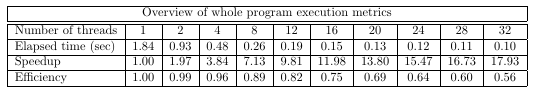
\includegraphics[width=0.9\linewidth]{fotosL4/primera_tabla_tree.png}
    \caption{Model factor 1 (Tree).}
    \label{fig:rec-tree-mf1}
\end{figure}

\begin{figure}[H]
    \centering
    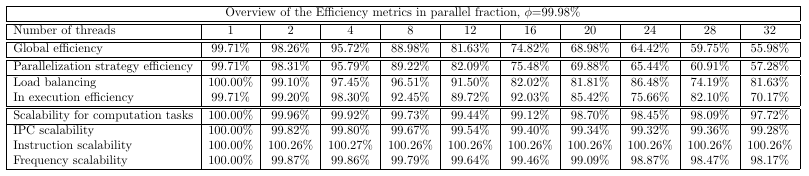
\includegraphics[width=0.9\linewidth]{fotosL4/segunda_tabla_tree.png}
    \caption{Model factor 2 (Tree).}
    \label{fig:rec-tree-mf2}
\end{figure}

\begin{figure}[H]
    \centering
    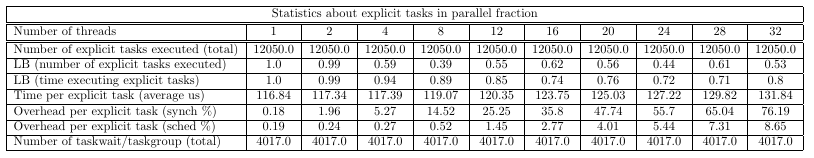
\includegraphics[width=0.9\linewidth]{fotosL4/tercera_tabla_tree.png}
    \caption{Model factor 3 (Tree).}
    \label{fig:rec-tree-mf3}
\end{figure}
A la primera taula destaca la millora en els resultats respecte les estratègies leaf. Veiem com l'Elapsed Time es redueix significativament, gairebé a la meitat els primers cops que dupliquem el nombre de threads, i que es redueix fins als 32 threads arrribant a un valor de 0.10 s, tot i així, a partir dels 16, la dismunució ja no és tan notoria.\\
Notem també que el SpeedUp millora molt sempre que augmentem el nombre de threads, son bons resultats, arribant a un Speedup de 17.93 amb 32 threads. Destaca també que l'Efficiency es manté força alta, major al 80\% fins als 12 threads i que en qualsevol cas, no baixa del 50\% en els casos estudiats.\\
Veiem a la segona taula que els valors de Load Balancing són molt millors que a la versió leaf, superiors al 90\% fins als 12 threads i després encara superiors al 80\%, cosa que indica que els threads estan molt ben equilibrats, i això es deu a què la creació de tasques es distribueix entre tots els threads disponibles.\\
Finalment, a la tercera taula destaca que el nombre de tasques executades és de 12015, molt superior al nombre de tasques executades a la versió leaf (gairebé quadriplicant), que era de 3013, i això es deu a què en aquesta versió es creen tasques per a totes les crides recursives, no només per a les fulles de l'arbre de recursió.\\

\subsection{Paraver Analysis}
\label{sec:rec-tree-paraver}

% Paraver trace (task creation / useful parallelism)
\begin{figure}[H]
    \centering
    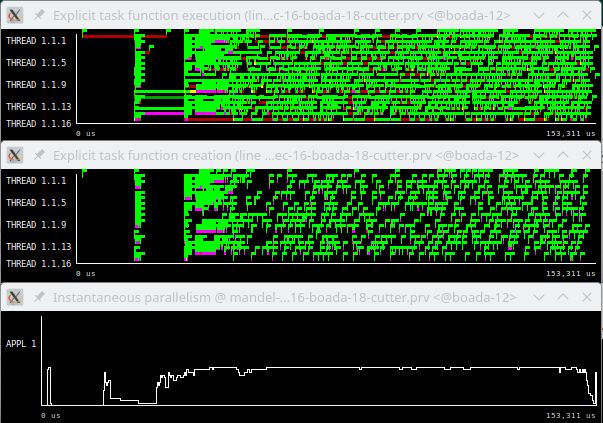
\includegraphics[width=0.9\linewidth]{fotosL4/paraver_tree.png}
    \caption{Paraver trace for Recursive Tree (16 threads): task density and execution.}
    \label{fig:rec-tree-paraver}
\end{figure}

A les traces obtingudes amb Paraver, podem observar el següent: d'una banda, veiem com tots els threads creen i executen tasques, a diferència de la versió leaf. Destaca també com inicialment, només un thread crea la tasca, hi ha un periode d'execució, en que no es creen ni s'executen tasques, i després, a mesura que es creen tasques, més threads s'incorporen a l'execució, i es van creant i executant tasques en paral·lel. Això es veu reflectit també en la densitat de tasques.
Veiem també, en relació a com s'inicia la creació de tasques, que a la traça inferior s'observa d'inici que es creen valls de threads actius, això es correspon amb el fet de que fins que no s'assoleix una certa profunditat en la recursió, no hi ha suficients tasques com per mantenir ocupats a tots els threads, però a mesura que es creen més tasques, més threads s'incorporen a l'execució. Destaca, en contrast amb l'estratègia leaf, que en el general de l'execució, l'ocupació dels threads roman molt més alta i estable.

\subsection{Strong Scalability}
\label{sec:rec-tree-scalability}

% Strong scalability plot
\begin{figure}[H]
    \centering
    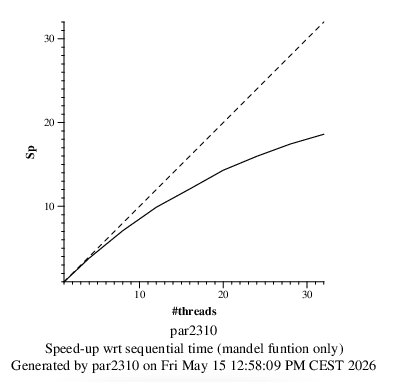
\includegraphics[width=0.75\linewidth]{fotosL4/grafico_tree.png}
    \caption{Strong scalability (elapsed time vs. threads) for the Recursive Tree implementation.}
    \label{fig:rec-tree-speedup}
\end{figure}
S'observa a la figura, tot i que ja s'ha esmentat, com l'SpeedUp millora molt en els primers increments del numero de threads, gairebé al ritme de la linia discontinua, però que a mesura que s'augmenta deixa d'augmentar tant notoriament l'SpeedUp.
Això s'analitza com que arriba un punt on afegir més threads no aporta tanta millora, ja que el nombre de tasques disponibles per executar no és suficient com per mantenir a tots ocupats, afegint a més més necesitat de sincronització entre threads.
\clearpage

% ==================================================================
\appendix
\chapter{Final Comparison Between All Parallel Strategies}
% ==================================================================

\section{Summary of Elapsed Execution Times}
\label{app:comparison}

Table~\ref{tab:elapsed} presents the elapsed execution times (in seconds) for all five
parallel versions, obtained from the output files generated by \texttt{submit-strong-omp.sh}.

\begin{table}[H]
\centering
\caption{Elapsed execution times (seconds) for each version and number of threads.}
\label{tab:elapsed}
\begin{tabular}{lcccccc}
\toprule
\textbf{Version} & \multicolumn{6}{c}{\textbf{Number of threads}} \\
\cmidrule(lr){2-7}
 & \textbf{1} & \textbf{4} & \textbf{8} & \textbf{12} & \textbf{16} & \textbf{32} \\
\midrule
Iterative: Tile (provided, completed)   & & & & & & \\
Iterative: Fine grain                   & & & & & & \\
Recursive: Leaf (provided, completed)   & & & & & & \\
Recursive: Improved Leaf                & & & & & & \\
Recursive: Tree                         & & & & & & \\
\midrule
\multicolumn{2}{l}{\textbf{Best parallel implementation}} &
\multicolumn{5}{l}{\textit{Version:} \quad \textit{Reason why:}} \\
\bottomrule
\end{tabular}
\end{table}

\section{Best Implementation Discussion}

% TODO: After filling in Table~\ref{tab:elapsed}, write 2--3 paragraphs discussing:
%   - Which iterative version is best and why (Tile vs. Fine grain).
%   - Which recursive version is best and why (Leaf, Improved Leaf, or Tree).
%   - Overall best implementation across both families.

\todo[inline]{Fill in Table~\ref{tab:elapsed} and write the discussion once experiments are complete.}

\end{document}
